\documentclass{article}

\usepackage{amsmath}
\usepackage{amssymb}
\usepackage{amsthm}
\usepackage{tikz}
\usepackage{listings}
\usepackage{hyperref}
\usepackage[margin=1in]{geometry}
\usepackage{xcolor}

\usetikzlibrary{arrows.meta, calc, 3d}

\definecolor{codebg}{rgb}{0.97,0.97,0.97}
\definecolor{codekw}{rgb}{0.10,0.30,0.65}
\definecolor{codecm}{rgb}{0.30,0.55,0.30}
\definecolor{codestr}{rgb}{0.65,0.10,0.10}

\lstset{
  language=JavaScript,
  basicstyle=\ttfamily\small,
  backgroundcolor=\color{codebg},
  keywordstyle=\color{codekw}\bfseries,
  commentstyle=\color{codecm}\itshape,
  stringstyle=\color{codestr},
  showstringspaces=false,
  breaklines=true,
  frame=single,
  numbers=left,
  numberstyle=\tiny,
  xleftmargin=2.5em,
  framexleftmargin=2em,
  morekeywords={THREE, Quaternion, Vector3, Euler, const, let}
}

\newtheorem{example}{Example}
\newtheorem{exercise}{Exercise}

\title{Guide 05: Quaternions and Axis--Angle\\
\large web-3d-panel-navigation math curriculum}
\author{}
\date{}

\begin{document}
\maketitle

\section{Why this matters}

Every tiled panel in this project gets its orientation from a quaternion
composition. The headliner is \texttt{resolveTiledPlane} in
\texttt{src/zoom-plane-parser.ts:421--475}: it builds a
\texttt{referenceQuaternion} from the parent panel's Euler rotation,
constructs a \texttt{relativeQuaternion} directly from an axis and a
``hinge angle'' (\texttt{data-tile-angle}), folds in an Euler-derived
\texttt{offsetQuaternion}, and multiplies the three together to get the
final orientation of the tiled panel. It then applies the result to
$(1,0,0)$ and $(0,1,0)$ to recover the rotated ``right'' and ``up''
basis vectors used to anchor the panel's position to the hinge edge.
That whole pipeline is what this guide is preparing you to read fluently.

\section{Building intuition: axis--angle}

The cleanest mental picture for a 3D rotation is \emph{axis--angle}: pick
a unit-length axis $\hat{\mathbf{n}}$, pick a signed angle $\theta$, and
rotate everything around that axis by that angle (right-hand rule). Every
rotation in 3D is some axis--angle pair. Euler angles are just a
particular bookkeeping for chaining three of them; a rotation matrix is
the linear map that one specific axis--angle produces.

\begin{center}
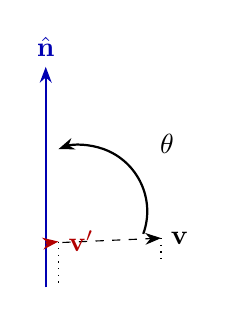
\begin{tikzpicture}[scale=1.4, >={Stealth[length=2mm]}]
  \draw[->, thick, blue!70!black] (0,-0.4,0) -- (0,1.6,0) node[above] {$\hat{\mathbf{n}}$};
  \draw[->, dashed] (0,0,0) -- (1.2,0.2,0.4) node[right] {$\mathbf{v}$};
  \draw[->, thick, red!70!black] (0,0,0) -- (0.5,0.4,1.0) node[right] {$\mathbf{v}'$};
  \draw[->, thick] (1.0,0.2,0.3) arc[start angle=-20, end angle=110, radius=0.6];
  \node at (1.1,0.9) {$\theta$};
  \draw[dotted] (1.2,0.2,0.4) -- (1.2,0,0.4);
  \draw[dotted] (0.5,0.4,1.0) -- (0.5,0,1.0);
\end{tikzpicture}
\end{center}

The vector $\mathbf{v}$ sweeps through angle $\theta$ around the axis
$\hat{\mathbf{n}}$. Components parallel to $\hat{\mathbf{n}}$ are
unchanged; components perpendicular to it rotate within the plane normal
to $\hat{\mathbf{n}}$.

This is exactly what \texttt{THREE.Quaternion.setFromAxisAngle} encodes,
and it is exactly the form the tiling code uses for its hinge:

\begin{lstlisting}
relativeQuaternion = new THREE.Quaternion().setFromAxisAngle(
  new THREE.Vector3(0, 1, 0),
  -layout.angle
);
\end{lstlisting}

``Spin around the world Y axis by $-\theta$.'' That's it. No matrices, no
Euler ordering convention, no ambiguity.

\section{The math}

\subsection{Definition}

A quaternion is a number of the form
\[
  q = w + x\,i + y\,j + z\,k
\]
where $i, j, k$ are imaginary units satisfying Hamilton's identity
\[
  i^2 = j^2 = k^2 = ijk = -1.
\]
This implies $ij = k$, $jk = i$, $ki = j$, and $ji = -k$, $kj = -i$,
$ik = -j$ (so quaternions are non-commutative).

We will write
\[
  q = (w, \mathbf{v}) \qquad \mathbf{v} = (x, y, z).
\]
\textbf{Three.js stores quaternions in the order $(x, y, z, w)$}; the
scalar part is last. Watch out for that mismatch when reading code or
debugging in the console.

\subsection{Multiplication (vector form)}

If you grind through Hamilton's identity, the product simplifies to
\[
  q_1 q_2 = \bigl(w_1 w_2 - \mathbf{v}_1 \cdot \mathbf{v}_2,\ \
              w_1 \mathbf{v}_2 + w_2 \mathbf{v}_1 + \mathbf{v}_1 \times \mathbf{v}_2\bigr).
\]
The cross product is what makes multiplication non-commutative: swapping
$q_1$ and $q_2$ flips the sign of $\mathbf{v}_1 \times \mathbf{v}_2$.

\subsection{The conjugate and the inverse}

The conjugate is
\[
  q^* = (w, -x, -y, -z).
\]
For a \emph{unit} quaternion ($w^2 + x^2 + y^2 + z^2 = 1$), the inverse is
just the conjugate:
\[
  q^{-1} = q^*.
\]
Every quaternion that represents a rotation is a unit quaternion, so in
this project we never compute a real inverse --- we only ever conjugate.

\subsection{The axis--angle correspondence (and the half-angle)}

A unit quaternion encodes axis--angle as
\[
  q = \bigl(\cos(\theta/2),\ \hat{\mathbf{n}} \sin(\theta/2)\bigr).
\]
The \emph{half}-angle is the strangest part of quaternions. Why $\theta/2$?

\paragraph{The double cover.} Plug in $\theta = 2\pi$ (a full
revolution): $\cos(\pi) = -1$, $\sin(\pi) = 0$, so
$q = (-1, \mathbf{0}) = -1$. A full $2\pi$ rotation gives $q = -1$, not
$q = +1$. You have to go around \emph{twice} (so $\theta = 4\pi$) to get
$q = +1$ back. Geometrically the rotation is the same after $2\pi$; the
quaternion has flipped sign. This is the famous fact that the unit
quaternions $S^3$ ``double cover'' the rotation group $SO(3)$:
\textbf{$q$ and $-q$ represent the same rotation}.

The half-angle is the price of admission for that double cover, and it
also makes the rotation formula clean:

\subsection{Rotating a vector}

Treat a 3D vector $\mathbf{v}$ as a pure quaternion $v = (0, \mathbf{v})$.
Then the rotated vector is
\[
  v' = q\, v\, q^{-1}.
\]
You can expand this and verify it matches the matrix Rodrigues formula
from guide~04, but in practice we let \texttt{applyQuaternion} do it:

\begin{lstlisting}
const newRight = new THREE.Vector3(1, 0, 0).applyQuaternion(quaternion);
\end{lstlisting}

That single line is the tiling code's way of asking ``what is the
panel's rotated $+x$ basis vector?''

\subsection{Composition order}

If you want to first rotate by $q_2$ and \emph{then} by $q_1$, the
combined rotation is
\[
  q_{\text{combined}} = q_1\, q_2.
\]
Reason: applying $q_{\text{combined}}$ to a vector gives
\[
  v' = (q_1 q_2)\, v\, (q_1 q_2)^{-1}
     = q_1\bigl(q_2\, v\, q_2^{-1}\bigr) q_1^{-1}.
\]
The inner conjugation $q_2 v q_2^{-1}$ runs first --- so $q_2$ is the
``inner'' (first) rotation and $q_1$ is the ``outer'' (second).

\paragraph{Three.js convention.} \texttt{Quaternion.multiplyQuaternions(a, b)}
sets \texttt{this = a * b}, and \texttt{q.multiply(other)} is the same as
\texttt{q.multiplyQuaternions(q, other)}. So
\begin{verbatim}
q.multiply(other)   // q := q * other
\end{verbatim}
post-multiplies. In the rotation interpretation, \texttt{other} is
applied first, then \texttt{q}. We will lean on this when we walk through
\texttt{resolveTiledPlane}.

\subsection{Why quaternions over Euler angles}

\begin{itemize}
\item \textbf{No gimbal lock.} The quaternion parameterization of $SO(3)$
is smooth (locally one-to-one up to the $\pm$ ambiguity). Euler angles
collapse a degree of freedom whenever the middle angle hits $\pm 90^\circ$.
\item \textbf{Clean composition.} Composing two rotations is one
quaternion product (16 multiplies, 12 adds) and the result is still
manifestly a rotation. Composing two Euler-angle triples requires
converting through matrices.
\item \textbf{Shortest-path interpolation.} Linearly interpolating Euler
angles produces non-uniform angular speed and bizarre paths. The
quaternion analogue, \emph{slerp}, traces the great-circle arc on $S^3$
and gives a constant-speed shortest-path rotation. We will use it in
guide 10.
\end{itemize}

\section{In this codebase}

All snippets are verbatim from
\texttt{src/zoom-plane-parser.ts:421--475}.

\subsection{Building the reference quaternion from Euler}

\begin{lstlisting}
const referenceQuaternion = new THREE.Quaternion().setFromEuler(
  new THREE.Euler(reference.rotation[0], reference.rotation[1], reference.rotation[2], 'XYZ')
);
const referenceRight = new THREE.Vector3(1, 0, 0).applyQuaternion(referenceQuaternion);
const referenceUp = new THREE.Vector3(0, 1, 0).applyQuaternion(referenceQuaternion);
\end{lstlisting}

\texttt{reference.rotation} is the parent panel's Euler triple
$(\alpha, \beta, \gamma)$ in radians, parsed from the
\texttt{data-rotation} attribute (see \texttt{ZoomPlaneConfig.rotation}
in \texttt{src/types.ts}). The \texttt{'XYZ'} order means: rotate by
$\alpha$ about $X$ first, then $\beta$ about $Y$, then $\gamma$ about
$Z$. The resulting quaternion is the product
$q_Z\, q_Y\, q_X$ where each factor is
$(\cos(\text{angle}/2), \hat{\mathbf{n}} \sin(\text{angle}/2))$ for the
respective axis.

The next two lines apply that quaternion to the world basis vectors
$\hat{\mathbf{x}}$ and $\hat{\mathbf{y}}$ to recover the panel's local
``right'' and ``up'' directions in world coordinates. By the rotation
formula, \texttt{referenceRight} is computing
$q\, (0, 1, 0, 0)\, q^{-1}$ and reading the vector part out. (Guide~06
will name this ``the panel's local frame.'')

\subsection{Direct axis--angle for the hinge}

\begin{lstlisting}
if (layout.side === 'right') {
  hinge = referenceCenter.clone().add(referenceRight.clone().multiplyScalar(reference.width * scale / 2));
  relativeQuaternion = new THREE.Quaternion().setFromAxisAngle(
    new THREE.Vector3(0, 1, 0),
    -layout.angle
  );
} else if (layout.side === 'left') {
  hinge = referenceCenter.clone().add(referenceRight.clone().multiplyScalar(-reference.width * scale / 2));
  relativeQuaternion = new THREE.Quaternion().setFromAxisAngle(
    new THREE.Vector3(0, 1, 0),
    layout.angle
  );
}
\end{lstlisting}

The tiled panel hinges around its shared edge with the reference panel.
For \texttt{side === 'right'}, the shared edge is the reference's right
edge --- a vertical line. We hinge \emph{around} that edge, which is a
rotation around (the reference's local) $Y$ axis. Note the code uses
the \emph{world} $Y$ axis $(0,1,0)$, not the reference's local up. That
is fine because \texttt{relativeQuaternion} will be composed
\emph{after} \texttt{referenceQuaternion} (we will see this below) and
post-composition is naturally interpreted in the reference's local
frame. More on that in a moment.

\paragraph{Why the sign flip?} Picture looking down the $+Y$ axis with
$+X$ to your right. A positive rotation around $+Y$ (right-hand rule)
spins points in the $XZ$ plane from $+X$ toward $-Z$. The right-side
neighbor panel, hinged on the right edge, must fold \emph{toward the
camera} (i.e.\ toward $+Z$). That is a \emph{negative} rotation around
$+Y$, hence \texttt{-layout.angle}. The left-side neighbor folds the
other way, so its sign is positive. Top/bottom use the $X$ axis with the
analogous sign convention.

\subsection{Composition of three quaternions}

\begin{lstlisting}
const offsetQuaternion = new THREE.Quaternion().setFromEuler(
  new THREE.Euler(
    layout.rotationOffset[0],
    layout.rotationOffset[1],
    layout.rotationOffset[2],
    'XYZ'
  )
);
const quaternion = referenceQuaternion.clone()
  .multiply(offsetQuaternion)
  .multiply(relativeQuaternion);
\end{lstlisting}

This is the heart of the pipeline. Recall \texttt{q.multiply(other)}
post-multiplies, so the resulting product is
\[
  q_{\text{final}} \;=\; q_{\text{ref}} \cdot q_{\text{offset}} \cdot q_{\text{rel}}.
\]
By the rule from \S 3.6, when applied to a vector, $q_{\text{rel}}$ acts
\emph{first}, then $q_{\text{offset}}$, then $q_{\text{ref}}$. Reading
the geometry that way:

\begin{enumerate}
\item \textbf{$q_{\text{rel}}$ first.} Take a panel sitting at the world
origin, axis-aligned. Hinge it around world $Y$ by $-\theta$. It is now
a panel in world space, tilted in the $XZ$ plane, but still attached to
``world'' axes.
\item \textbf{Then $q_{\text{offset}}$.} Apply the small Euler-derived
adornment rotation. Because we have only applied $q_{\text{rel}}$ so
far, this offset is composed in the rel-rotated frame from the previous
step.
\item \textbf{Then $q_{\text{ref}}$.} Now reorient the whole assembly
into the reference panel's frame. Equivalently: the hinge angle that we
specified ``around world $Y$'' becomes a hinge around \emph{the
reference's local $Y$} after this final rotation, which is exactly what
``hinge around the shared edge'' means geometrically.
\end{enumerate}

The test suite confirms this composition explicitly
(\texttt{src/zoom-plane-parser.test.ts:533--543}):

\begin{lstlisting}
const referenceQuaternion = quaternionFromConfig(referenceConfig);
const offsetQuaternion = new THREE.Quaternion().setFromEuler(
  new THREE.Euler(0, 2 * Math.PI / 180, -Math.PI / 180, 'XYZ')
);
const foldQuaternion = new THREE.Quaternion().setFromAxisAngle(
  new THREE.Vector3(0, 1, 0),
  -35 * Math.PI / 180
);
const expectedQuaternion = referenceQuaternion.clone()
  .multiply(offsetQuaternion)
  .multiply(foldQuaternion);
\end{lstlisting}

\subsection{Reading off the rotated basis}

\begin{lstlisting}
const newRight = new THREE.Vector3(1, 0, 0).applyQuaternion(quaternion);
const newUp = new THREE.Vector3(0, 1, 0).applyQuaternion(quaternion);
\end{lstlisting}

These two lines compute, for the final tiled panel,
\[
  \texttt{newRight} = q_{\text{final}}\,(0,1,0,0)\,q_{\text{final}}^{-1}, \qquad
  \texttt{newUp}    = q_{\text{final}}\,(0,0,1,0)\,q_{\text{final}}^{-1},
\]
reading out the vector parts. The position of the panel's center is
then \texttt{hinge + newRight * width/2} (or its mirror), so the panel
butts up against the hinge edge along its own rotated right axis. This
is the practical reason we cared about the rotated basis at all: the
panel's geometric center is offset from the hinge along the panel's
local right or up direction, which in world coordinates is
\texttt{newRight} or \texttt{newUp}.

\section{Worked examples}

\begin{example}\label{ex:axis-angle}
A panel has \texttt{data-tile-angle="30"} and tiles to the
\texttt{right}. Compute its \texttt{relativeQuaternion}.

\medskip
\textbf{Solution.} The angle in radians is
$\theta = 30^\circ \cdot \pi/180 = \pi/6$. The code negates this for the
right side, so the actual rotation is $-\pi/6$ around $\hat{\mathbf{y}}$:
\[
  q_{\text{rel}} = \bigl(\cos(-\pi/12),\ (0,1,0)\sin(-\pi/12)\bigr)
                 = (\cos 15^\circ,\ 0,\ -\sin 15^\circ,\ 0)
\]
Numerically, $\cos 15^\circ \approx 0.9659$, $\sin 15^\circ \approx 0.2588$, so
\[
  q_{\text{rel}} \approx (0.9659,\ 0,\ -0.2588,\ 0).
\]
In Three.js storage order $(x, y, z, w)$, that is
$(0,\ -0.2588,\ 0,\ 0.9659)$.
\end{example}

\begin{example}\label{ex:compose}
The reference panel has \texttt{data-rotation="0, 45, 0"} (degrees).
Ignore \texttt{rotationOffset} (so $q_{\text{offset}} = 1$). Compute the
composed quaternion for the right-side tile from
Example~\ref{ex:axis-angle}.

\medskip
\textbf{Solution.} The reference quaternion is a $45^\circ$ rotation
around $Y$:
\[
  q_{\text{ref}} = (\cos 22.5^\circ,\ 0,\ \sin 22.5^\circ,\ 0)
                 \approx (0.9239,\ 0,\ 0.3827,\ 0).
\]
Both $q_{\text{ref}}$ and $q_{\text{rel}}$ are pure-Y rotations, so they
commute and add in the angle: total angle around $Y$ is
$45^\circ + (-30^\circ) = 15^\circ$. So
\[
  q_{\text{final}} = (\cos 7.5^\circ,\ 0,\ \sin 7.5^\circ,\ 0)
                   \approx (0.9914,\ 0,\ 0.1305,\ 0).
\]
You can also verify this by the vector multiplication formula in \S 3.2:
since $\mathbf{v}_1 \cdot \mathbf{v}_2 = 0 \cdot 0 + a\cdot b + 0\cdot 0 = ab$
where $a = \sin 22.5^\circ$, $b = -\sin 15^\circ$, and the cross
product of two vectors both pointing along $\hat{\mathbf{y}}$ is zero, the
product reduces to scalar arithmetic that matches the half-angle sum.
\end{example}

\begin{example}\label{ex:basis}
Using $q_{\text{final}}$ from Example~\ref{ex:compose}, predict
\texttt{newRight}.

\medskip
\textbf{Solution.} A pure rotation by $15^\circ$ around $\hat{\mathbf{y}}$
takes $\hat{\mathbf{x}} = (1,0,0)$ to
\[
  (\cos 15^\circ,\ 0,\ -\sin 15^\circ) \approx (0.9659,\ 0,\ -0.2588).
\]
Sanity check: this points slightly into $-Z$ (toward the camera) and
mostly along $+X$, exactly what you would expect for a panel that has
been folded $15^\circ$ in the right-folding direction relative to the
world axes.
\end{example}

\section{Exercises}

\begin{exercise}\label{ex1}
Write the unit quaternion for a $90^\circ$ rotation around $\hat{\mathbf{z}}$.
Give it both as $(w, x, y, z)$ and in Three.js storage order.
\end{exercise}

\begin{exercise}\label{ex2}
Write the unit quaternion for a $180^\circ$ rotation around the unit
axis $\hat{\mathbf{n}} = \frac{1}{\sqrt{2}}(1, 1, 0)$.
\end{exercise}

\begin{exercise}\label{ex3}
\textbf{Conceptual.} Show that $-q$ represents the same rotation as $q$,
by plugging $-q$ into the rotation formula $v' = q v q^{-1}$ and showing
the result is unchanged.
\end{exercise}

\begin{exercise}\label{ex4}
Two quaternions $q_1 = (\cos 30^\circ, \hat{\mathbf{x}} \sin 30^\circ)$ and
$q_2 = (\cos 30^\circ, \hat{\mathbf{y}} \sin 30^\circ)$ represent
$60^\circ$ rotations around $\hat{\mathbf{x}}$ and $\hat{\mathbf{y}}$
respectively. Compute $q_1 q_2$ and $q_2 q_1$ using the vector-form
multiplication rule. They should differ --- the cross-product term
$\mathbf{v}_1 \times \mathbf{v}_2$ flips sign.
\end{exercise}

\begin{exercise}\label{ex5}
\textbf{Project-applied.} The reference plane has rotation
$(0,\ 90^\circ,\ 0)$ and we tile to the right at \texttt{data-tile-angle="45"}.
Predict \texttt{newRight}. (Hint: total $Y$ rotation is
$90^\circ + (-45^\circ) = 45^\circ$.) Sketch where the tiled panel sits
relative to the reference panel.
\end{exercise}

\subsection*{Extension challenges}

\begin{exercise}\label{exA}
Show that the cosine of the angle between two rotations $q_a$ and $q_b$
(as a single ``angular distance'') is $|q_a \cdot q_b|$ (treating
quaternions as 4-vectors and dotting them). Why the absolute value?
Connect this to the helper \texttt{expectQuaternionClose} in
\texttt{src/zoom-plane-parser.test.ts:43--45}, which checks
\texttt{Math.abs(actual.dot(expected))} is close to 1.
\end{exercise}

\begin{exercise}\label{exB}
Suppose a hypothetical refactor wrote the composition as
\texttt{relativeQuaternion.clone().multiply(offsetQuaternion).multiply(referenceQuaternion)}
instead. Describe geometrically what would go wrong, in terms of which
frame each rotation gets interpreted in.
\end{exercise}

\section{Where to next}

Guide 06 picks up the loose end we kept dropping: ``the panel's local
frame.'' That guide will define a frame as a triple of orthonormal basis
vectors (right, up, normal) and tie it to both the rotation matrix
picture from guide 04 and the quaternion picture here. The line
\texttt{new THREE.Vector3(1,0,0).applyQuaternion(q)} is exactly the
quaternion-side computation of the local right basis vector.

Guide 10 will introduce \emph{slerp}, the constant-angular-speed
interpolation between two quaternions, which is what you would reach for
if you wanted to animate a panel from one orientation to another along
the shortest arc.

\section*{Appendix: Solutions}

\paragraph{Exercise~\ref{ex1}.} A $90^\circ$ rotation around
$\hat{\mathbf{z}}$ has half-angle $45^\circ$:
\[
  q = (\cos 45^\circ,\ 0,\ 0,\ \sin 45^\circ)
    = \tfrac{1}{\sqrt{2}}\,(1,\ 0,\ 0,\ 1).
\]
In Three.js storage $(x, y, z, w)$ that is
$\bigl(0,\ 0,\ \tfrac{1}{\sqrt{2}},\ \tfrac{1}{\sqrt{2}}\bigr)$.

\paragraph{Exercise~\ref{ex2}.} Half-angle $90^\circ$, so $\cos = 0$,
$\sin = 1$. The vector part is $\hat{\mathbf{n}}\sin 90^\circ = \hat{\mathbf{n}}$:
\[
  q = \bigl(0,\ \tfrac{1}{\sqrt{2}},\ \tfrac{1}{\sqrt{2}},\ 0\bigr)
\]
in $(w, x, y, z)$ form.

\paragraph{Exercise~\ref{ex3}.} Substituting $-q$ into the rotation:
\[
  (-q)\, v\, (-q)^{-1} = (-q)\, v\, (-q^{-1}) = (-1)(-1)\, q\, v\, q^{-1} = q\, v\, q^{-1}.
\]
The two minus signs cancel; same rotation. (We used
$(-q)^{-1} = -q^{-1}$, which holds because
$(-q)(-q^{-1}) = q\,q^{-1} = 1$.)

\paragraph{Exercise~\ref{ex4}.} With $\mathbf{v}_1 = (\sin 30^\circ, 0, 0)$,
$\mathbf{v}_2 = (0, \sin 30^\circ, 0)$, and $w_1 = w_2 = \cos 30^\circ$:
\begin{align*}
\mathbf{v}_1 \cdot \mathbf{v}_2 &= 0 \\
\mathbf{v}_1 \times \mathbf{v}_2 &= (0, 0, \sin^2 30^\circ) = (0, 0, 0.25) \\
q_1 q_2 &= \bigl(\cos^2 30^\circ,\ \cos 30^\circ \cdot (0, \sin 30^\circ, 0) + \cos 30^\circ \cdot (\sin 30^\circ, 0, 0) + (0, 0, 0.25)\bigr) \\
        &= \bigl(0.75,\ \tfrac{\sqrt{3}}{4},\ \tfrac{\sqrt{3}}{4},\ 0.25\bigr).
\end{align*}
For $q_2 q_1$ the cross product is $\mathbf{v}_2 \times \mathbf{v}_1 = (0, 0, -0.25)$,
so
\[
  q_2 q_1 = \bigl(0.75,\ \tfrac{\sqrt{3}}{4},\ \tfrac{\sqrt{3}}{4},\ -0.25\bigr).
\]
Different rotations, as expected.

\paragraph{Exercise~\ref{ex5}.} The reference is rotated $90^\circ$
around $Y$, so its local right is
$(1,0,0)$ rotated by $90^\circ$ around $Y$, i.e.\ $(0, 0, -1)$. The
tile's \texttt{relativeQuaternion} is $-45^\circ$ around $Y$. The total
$Y$ rotation in the composed quaternion is $45^\circ$, so
$\texttt{newRight} = (1,0,0)$ rotated $45^\circ$ around $Y$:
\[
  \texttt{newRight} = (\cos 45^\circ, 0, -\sin 45^\circ)
                    \approx (0.707,\ 0,\ -0.707).
\]
Geometrically: the reference panel faces $+X$ (its surface normal points
along $+X$ after the $90^\circ$ Y rotation). The right tile hinges from
the reference's right edge --- which is at $-Z$ relative to the
reference center --- and folds halfway between the reference's plane
and the world $-Z$ direction.

\paragraph{Exercise~\ref{exA}.} Treating $q_a, q_b$ as unit 4-vectors,
their dot product equals $\cos(\Theta/2)$ where $\Theta$ is the angle of
the relative rotation $q_a^{-1} q_b$. Two quaternions that differ only
in sign represent the same rotation but have dot product $-1$ rather
than $+1$, so the absolute value collapses the double-cover ambiguity.
The test helper \texttt{expectQuaternionClose} checks
\texttt{Math.abs(actual.dot(expected))} is close to 1, which is exactly
the condition ``these two quaternions represent the same rotation,
modulo sign.''

\paragraph{Exercise~\ref{exB}.} Reversing the order to
$q_{\text{rel}} \cdot q_{\text{offset}} \cdot q_{\text{ref}}$ would mean
$q_{\text{ref}}$ is applied \emph{first} and $q_{\text{rel}}$ is applied
\emph{last}, in the original world frame. The hinge rotation around
world $Y$ would then be applied after the reference orientation is
already baked in --- so the panel would hinge around the world $Y$ axis
through the origin instead of around the reference's local up axis
through the shared edge. Visually: tilted reference panels would have
their tiles fold incorrectly, drifting off the shared edge.

\end{document}
